% Metódy inžinierskej práce

\documentclass[10pt,twoside,slovak,a4paper]{article}

\usepackage[slovak]{babel}
%\usepackage[T1]{fontenc}
\usepackage[IL2]{fontenc} % lepšia sadzba písmena Ľ než v T1
\usepackage[utf8]{inputenc}
\usepackage{graphicx}
\usepackage{url} % príkaz \url na formátovanie URL
\usepackage{hyperref} % odkazy v texte budú aktívne (pri niektorých triedach dokumentov spôsobuje posun textu)
\usepackage{cite}
%\usepackage{times}
%\pagestyle{headings}

\title{Virtuálna realita, modelovanie a simulácia v oblasti medicíny 
\thanks{Semestrálny projekt v predmete Metódy inžinierskej práce, ak. rok 2021/22, vedenie: Ing. Fedor Lehocki, PhD.}} % meno a priezvisko vyučujúceho na cvičeniach

\author{Matúš Stankovič\\[2pt]
	{\small Slovenská technická univerzita v Bratislave}\\
	{\small Fakulta informatiky a informačných technológií}\\
	{\small \texttt{xstankovic@stuba.sk}}
	}

\date{\small 20. október 2021} % upravte



\begin{document}

\maketitle

\begin{abstract}
V informatike prebieha rýchli a neustály vývoj. Pokroky vo výpočtovom výkone umožňujú 
implikovanie informatiky do čoraz väčšieho spektra rôznych oborov. V posledných rokoch sa 
rapídne vyvinula aj oblasť virtuálnej reality, ktorá našla uplatnenie v rôznorodých oblastiach. 
Medicína je jednou z oblastí kde virtuálna realita zožala veľký úspech. V mojej práci by som sa chcel 
venovať uplatneniu virtuálnej reality, modelovaniu a simulácii v medicíne. Či už je to 
využitie softvérových 3D modelov ľudského tela, orgánov a tkaniva pri vzdelávaní študentov, 
využitie simulácie operácii pre vzdelávanie, ale aj pre samotné predoperačné plánovanie a 
tréning chirurgov\ldots
\end{abstract}



\section{Úvod}
Medicína je zložitá a dôsledná vedná disciplína. S pokrokom doby a vývojom nových technológii, bolo potrebné modernizovať aj medicínu~\ref{modelovanie}. Vzdelávanie v medicíne malo už dlhšie časové obdobie isté úskalia.

Podstatným problémom pre vzdelávanie chirurgov~\ref{chirurgia}, ale aj iných medicínskych odvetví, boli neefektívne výučbové procesi. Bolo a je to zapríčinené nedostatkom ľudí ktorí sú ochotný darovať svoje telo, po smrti, na medicínske účely. Toto viedlo k vytváraniu náučných videí a výučbových publikácii, ktoré však študentom nepribližujú reálne praktické zručnosti. Preto bolo implementovanie 3D modelovania, simulácie a virtuálnej reality do tohto oboru veľkým prínosom. Vvyužíva sa na výučbu študentov~\ref{vzdelanie}, kde môže nahradiť výuku na ľudskom tele ktorá je menej efektívna. Modelovanie a virtuálna realita je tiež veľmi nápomocná pri stanovení diagnózy, predoperačnej príprave, pri chirurgických zákrokoch, používa sa taktiež pri liečbe a procedúrach, taktiež sa používa na terapeutické účely.

Keďže medicína sa nás všetkých viac či menej dotýka rozhodol som sa v tomto článku priblížiť implementáciu informatiky, a to hlavne virtuálnej reality, simulácie a 3D modelov do medicínskeho prostredia.  


\section{Modelovanie v softvérovom inžinierstve} \label{modelovanie}
Pri modelovaní poznáme rôzne techniky, uplatňujúce sa v rôznych odboroch. Modelovanie v softvérovom inžinierstve predstavuje priebeh vytvorenia softvérového prototypu, modelu, ktorý slúži na zjednodušenie, odhalenie efektivity modelovaného problému. Vytvorenie modelu môžeme chápať ako predprípravu na riešenie akéhokoľvek požadovaného problému. Pri modelovaní sa berú v úvahu rôzne aspekty ovplyvňujúce danú problematiku čo prináša veľké výhody, pretože už pred realizáciou riešenia daného problému, môžu byť v modelovej implementácii odhalené rôzne nedostatky a nepredvídané komplikácie. 

\begin{figure*}[tbh]
\centering
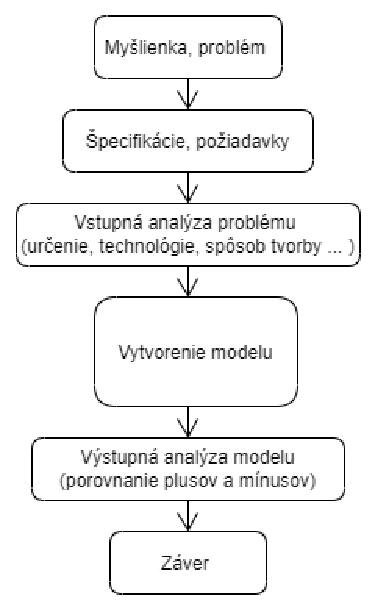
\includegraphics[scale=1.0]{diagram.pdf}
\caption{Tvorba modelu.}
\label{f:model}
\end{figure*}

Softvérové modelovanie sa využíva v rôznorodých oblastiach. Môže byť napríklad použité pri modelovaní virtuálnej reality v spojení s vytváraním modelov v stavebníctve, strojárstve, letectve, v medicíne, ale aj vo veľkom počte iných odvetví. V medicíne má softvérové modelovanie rôznorodé uplatnenie, v rôznich formách, ide napríklad o 3D modely ľudského tela, orgánov, tkanív, modelovanie sa tiež využíva pri simuláciach operačných zákrokov, liečbe diagnóz, predoperačných prípravách. Taktiež virtuálna realita sa v medicíne používa na výučbu a prípravu študentov, na tréning chirurgov a ich prípravu, ale aj na liečbu diagnóz a terapie. \cite{2018}   


\section{Vzdelávanie pomocou modelovania } \label{vzdelanie}
Významným problémom vo výučbe medicíny sa stal neefektívny proces výučby, ktorý bol spôsobený nedostatkom darcov tiel pre výučbu. Taktiež veľkým nedostatkom je aj uchovávanie týchto výučbových pomôcok, či už mrazením alebo iným konzervovaním, pretože po takomto uchovaní stráca telo reálne vlastnosti ktoré sú veľmi dôležité pre výučbu. Všetky tieto nedostatky dokáže odstrániť modelovanie a virtuálna realita. Pomocou nich je možné vytvoriť dokonalé modely ľudských orgánov, tkanív, svalstva, kostí a celej anatómie tela, umožnuje demonštrovať ich skutočné správanie a fungovanie. Modely a virtuálna realita dokážu dôveryhodne reprezentovať nie len zdravé orgány a tkanivá, ale taktiež konkrétne správanie chorých a v nadveznosti na to dokážu vyobrazovať aj ich správanie počas liečby. \cite{2016}   



\section{Modelovanie a chirurgia} \label{chirurgia}
Zavedenie moderných praktík, ako je simulácia, virtuálna realita a 3D modely, do procesu výučby a opakovaných kurzov chirurgie prinieslo pokrok v efektivite a precíznosti odborníkov pracujúcich v tomto odvetví. Výskum potvrdil že študenti ktorý boli vzdelávaní pomocou simulácie vo virtuálnej realite sú efektívnejší, rýchlejší, precíznejší a do reálnych zákrokov vstupujú s väčšou istotou. \cite{2016}  

\subsection{Model SDK} \label{SDK}

\section{Rehabilitácie a terapie} \label{rehab}
Virtuálna realita prináša aj do oboru terapie a rehabilitácii veľký prínos. Je využívaná pri terapiách s pacientami ktorí trpia mentálnym ochorením, psichyckými poruchami, traumami, ale tiež sa využíva aj pri rehabilitáciach ľudí ktorý prekonali mŕtvicu. \cite{2020}  

\section{Záver} \label{zaver} % prípadne iný variant názvu



% týmto sa generuje zoznam literatúry z obsahu súboru literatura.bib podľa toho, na čo sa v článku odkazujete
\bibliography{literatura}
\bibliographystyle{plain} % prípadne alpha, abbrv alebo hociktorý iný
\end{document}
